\chapter{Листинг программы}

На листинге \ref{lst3} показан код программы, выводящий агрумент с результатами работы методов, которые необходимо было реализовать по условию лабораторной.

\begin{lstlisting}[caption=код программы, label=lst3]

static class Methods
    {
        public static double f(double x, double y) 
        {
            return (Math.Pow(x, 2) + Math.Pow(y, 2));
        }
        public static double EulerOpened(double x, double h, double y) 
        { 
            return y + h * f(x, y);
        }

        public static double Pikar(double x, int n) 
        {
            
            switch (n)
            {
                case 1:
                    return Math.Pow(x, 3) / 3;
                case 2:
                    return Math.Pow(x, 3) / 3 + Math.Pow(x, 7) / 63;
                case 3:
                    return Math.Pow(x, 3) / 3 + Math.Pow(x, 7) / 63 + 2 * Math.Pow(x, 11) / 2079 + Math.Pow(x, 15) / 59535;
                case 4:
                    return Math.Pow(x, 3) / 3 + Math.Pow(x, 7) / 63 + 2 * Math.Pow(x, 11) / 2079 + 13 * Math.Pow(x, 15) / 218295 + 82 * Math.Pow(x, 19) / 37328445 + 662 * Math.Pow(x, 23) / 10438212015  + 4 * Math.Pow(x, 27) / 3341878155 +  Math.Pow(x, 31) / 109876902975;
                default:
                    return Math.Pow(x, 3) / 3;
            }
        }

        public static double Runge(double x, double y, double h)
        {
            var alpha = 0.5;
            var k1 = Methods.f(x, y);
            var k2 = f(x + h / 2 / alpha, y + k1 * h / 2 / alpha);
            y = y + h * ((1 - alpha) * k1 + alpha * k2);
            return y;
        }
        
    }

class Program
    {
        static void Main()
        {
            Console.Write("Enter xMax:");
            var xMax = double.Parse(Console.ReadLine());

            Console.Write("Enter step:");
            var h = double.Parse(Console.ReadLine());

            Console.Write("Enter Pikard approximation:");
            var n = int.Parse(Console.ReadLine());

            double EulerOpened_y = 0;
            double Pikar_y;
            double Runge_y = 0;

            double x0 = 0;
            Console.WriteLine($"      X       Euler      Pikard{n}    Runge");
            while (x0 < xMax + h)
            {
                EulerOpened_y = Methods.EulerOpened(x0, h, EulerOpened_y);
                Runge_y = Methods.Runge(x0, Runge_y, h);
                Pikar_y = Methods.Pikar(x0, n);
                Console.WriteLine("{0,6:F8}|{1,6:F8}|{2,6:F8}|{3,6:F8}|", x0, EulerOpened_y, Pikar_y, Runge_y);
                x0 += h;
            }
    }
   
\end{lstlisting}

На рисунках \ref{fig:fig2} и \ref{fig:fig3} показан вывод программы со значениями аргументов и результатом работы методов с этими аргументами.

\begin{figure}[ht!]
  \centering
  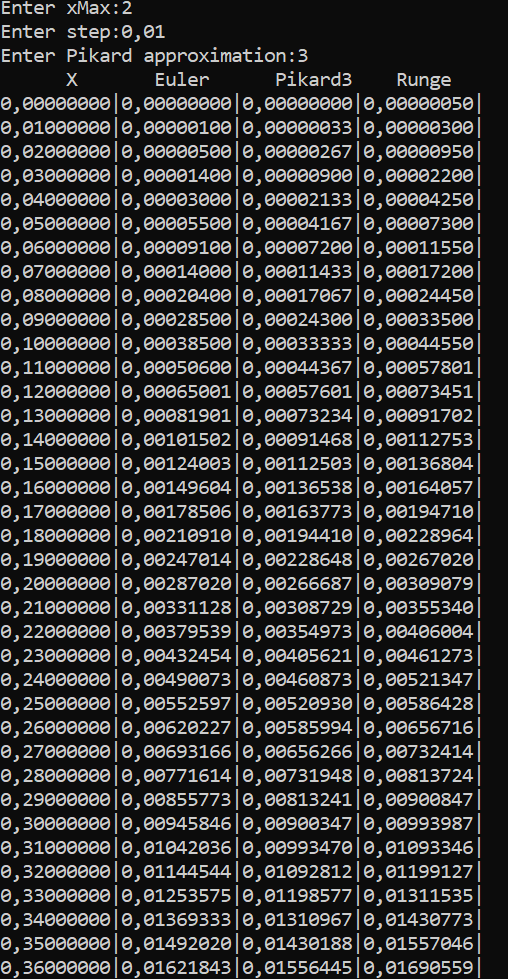
\includegraphics[scale=1]{img/result_table1.png}
  \caption{вывод программы}
  \label{fig:fig2}
\end{figure}

\begin{figure}[ht!]
  \centering
  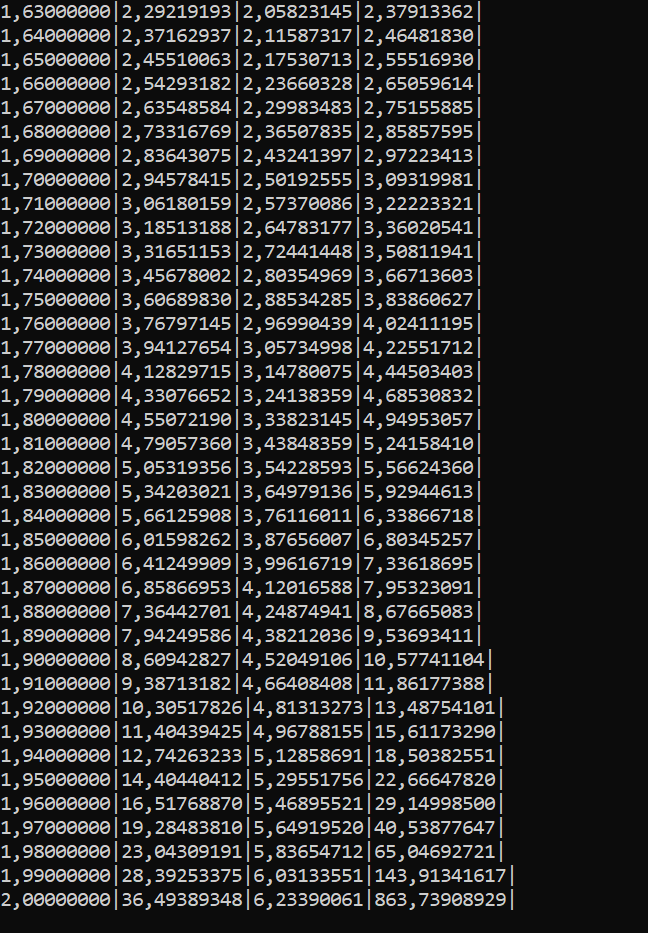
\includegraphics[scale=1]{img/result_table2.png}
  \caption{вывод программы}
  \label{fig:fig3}
\end{figure}

\newpage